\documentclass{article}
\usepackage[T1]{fontenc}
\usepackage{lmodern}
\usepackage{graphicx}
\usepackage{amsmath,amssymb}
\usepackage[a4paper,margin=2cm]{geometry}
\usepackage[absolute,overlay]{textpos}
\setlength{\TPHorizModule}{1mm}
\setlength{\TPVertModule}{1mm}
\usepackage[indonesian]{babel}
\usepackage{hyperref}
\setlength{\emergencystretch}{2em}
% unit: Halaman 17

\begin{document}

% === Halaman 17 (llm) ===

yang dalam hal ini nilai $P_w$ dan $Q_w$ (dalam heksadesimal) berbeda-beda bergantung pada $w$ sebagai berikut [STA98]:

\vspace{10mm}

Konstanta $P_w$ dan $Q_w$ didasarkan pada representasi bilangan alam $e$ dan $\phi$ dalam biner,

\begin{align*}
P_w &= \text{Odd}[(e-2)2^w] \\
Q_w &= \text{Odd}[(\phi-1)2^w]
\end{align*}

\vspace{20.20mm}

yang dalam hal ini,

\[ e = 2.718281828459... \]
\[ \phi = 1.618033988749... = \frac{1+\sqrt{5}}{2} \]

% deskripsi: Tabel nilai Pw dan Qw dalam heksadesimal untuk berbagai nilai w (16, 32, 64).
% bbox normalisasi: [0.1560, 0.2500, 0.8420, 0.4060]
\begin{textblock*}{144.06mm}(32.76mm,74.25mm)
\noindent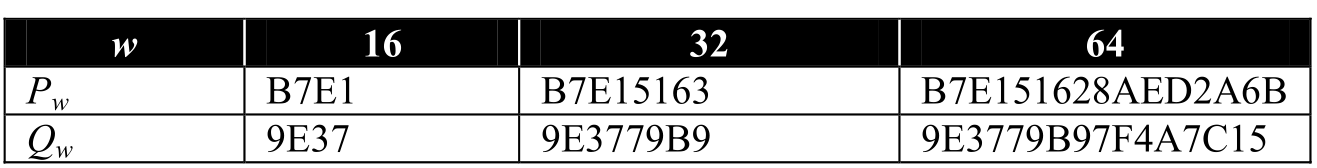
\includegraphics[width=144.06mm,height=46.33mm]{../../images/llm/page_017_img_01.png}%
\end{textblock*}

% deskripsi: Teks berwarna merah yang menjelaskan definisi fungsi Odd sebagai fungsi yang memberikan integer ganjil terkecil yang dekat dengan input yang diberikan.
% bbox normalisasi: [0.4170, 0.5850, 0.9010, 0.6530]
\begin{textblock*}{101.64mm}(87.57mm,173.74mm)
\noindent
\includegraphics[width=101.64mm,height=20.20mm]{../../images/llm/page_017_img_02.png}%
\end{textblock*}

\end{document}
